\section{The Applications of SNIPER Framework} \label{sec:SNIPERResults}
In this section, we showcase the effectiveness of SNIPER for two main applications, namely per-flow delay and per-flow size estimations, and under different configurations. Each configuration determines the network under study, the matrix completion technique, the length of learning period $T_{0}$, and the sampling ratio $s$. Here, $T$ is set to $T=100$; however, $s$ mainly varies in the range of small values to indicate a case of hard constraint of network measurement resources. Other parameters, such as the number of measurement paths $K$ and the number of parts in the data set $t_{p}$ can be determined, accordingly. The type of sampling strategies are denoted by RS, GA and PSO which respectively identify the OOM designed by Random Sampling (RS) and evolutionary algorithms GA or PSO. Note that, the performance of RS strategy is evaluated using Monte-Carlo simulation with 100 iterations. 
% The type of the sampling strategy that is used to identify the ONMP in the SNIPER framework is another parameter that is used in the definition of each configuration. The sampling strategies are identified by notions RS, GA and PSO which respectively denote the ONMP designed by random sampling and evolutionary algorithms GA or PSO. Note that the performance of the following results can be improved by increasing the number generations in the evolutionary algorithms.
% **** Add the parameters of GA and PSO ****
%Each configuration defines how the measurement process is setup in the SNIPER framework and how it evaluates the performance of the estimation. 

\subsection{Optimal Observation Matrix Design using SNIPER}
The optimal design of large-scale binary observation matrices, using mathematical optimization techniques are extremely complicated or computationally expensive. Here, to show the effectiveness of our evolutionary OOM design, we consider a small ring network consisting of 4 nodes with different per-flow path delays where we can compute all possible observation matrices at a specific sampling ratio. Then, we estimate the unobserved entries and compute the corresponding NMSE for all possible observation matrices. Using this process we realized that our EOAs are able to obtain the OOM. As an example, if $X=[0,5.05,9.01,9.645;5.05,0,3.96,9.645;9.01,3.96,0,5.23; \\ 4.595,9.645,5.23,0]$ (in ms) and $s=0.25$, then the OOM $S_{\Omega}^{Opt}(X)$ with $NMSE=0.4734$ is $S_{\Omega}^{Opt}(X)=[0,0,1,0;0,0,0,1;1,0,0,0;0,1,0,0]$ which is also obtained by our GA in SNIPER framework.

\subsection{Per-Flow Delay Estimation using SNIPER}
Figures \ref{fig:AbileneGADelayNoise} and \ref{fig:GeantGADelayNoise} show the performance of the SNIPER in the estimation of per-flow delay on Abilene and Geant networks using synthesis data generated using the model in Eq.(\ref{DelayModel}) where the MC technique is DMFSGD as in \cite{YLiao:2011}. Here, the OOM is designed using the GA and only by considering the propagation delay in Eq.(\ref{DelayModel}) in the learning epoch. Then, this OOM is used to evaluate the performance of the MC technique in measurement epochs, based on the $NMSE_{Avg}$, where queuing delay is added to the propagation delay as Eq.(\ref{DelayModel}) models the network paths delay \cite{Pietro:2008}. Figure \ref{fig:HarvardGADelayNoise} also shows the performance of the SNIPER framework on real per-flow delay from Harvard \cite{JLedlie:2007} network. In this figure, and throughout this paper, the blue squares represent the minimum and maximum of $NMSE$ or (or $NMAE$) for each sampling ratio using our EOA based sampling strategy.  It should be noted that, in low sampling ratios and in all measurement epochs a better estimation accuracy is obtained comparing with random sampling strategy. In addition, Table \ref{tab:PdfaHarvard} indicates the capability of the SNIPER framework in the reliable detection of Congested Paths (CP). These results show that, at lower SRs which indicates the hard resource constraint regime, by the intelligent design of the OOM messages using the SNIPER framework a better estimation accuracy, with more robust performance against noise, can be obtained via applying MC techniques. This is an important factor in active network performance measurement, including delay, where the communication bandwidth is the main resource for accurate measurement and it is very limited.

% (equivalent results were obtained for Geant network)
% Comparing with the random sampling, this figure show that for lower SRs, the ONMP designed by the GA provides better estimation accuracy. Also it is more robust against the variance of the queuing delay. This is an important factor for active network measurements under hard resource constraints. 
\begin{figure*} % 30  33
  \begin{center}
\minipage{0.21\textwidth}
  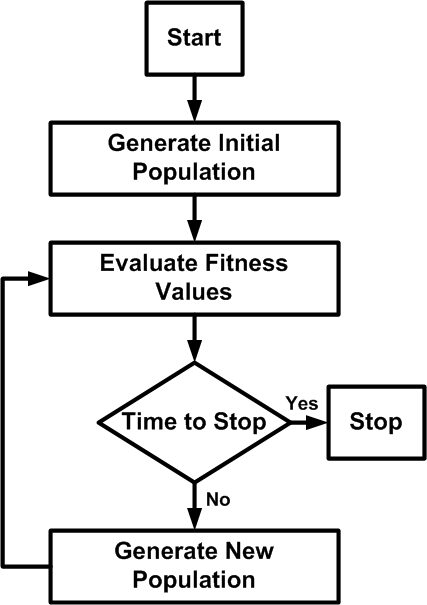
\includegraphics[width=\linewidth]{EvolutionaryAlgsFC.png}
  \caption{{The flowchart of evolutionary optimization algorithms.}}\label{fig:EvolutionaryAlgsFC}
\endminipage\hfill
\minipage{0.36\textwidth}
  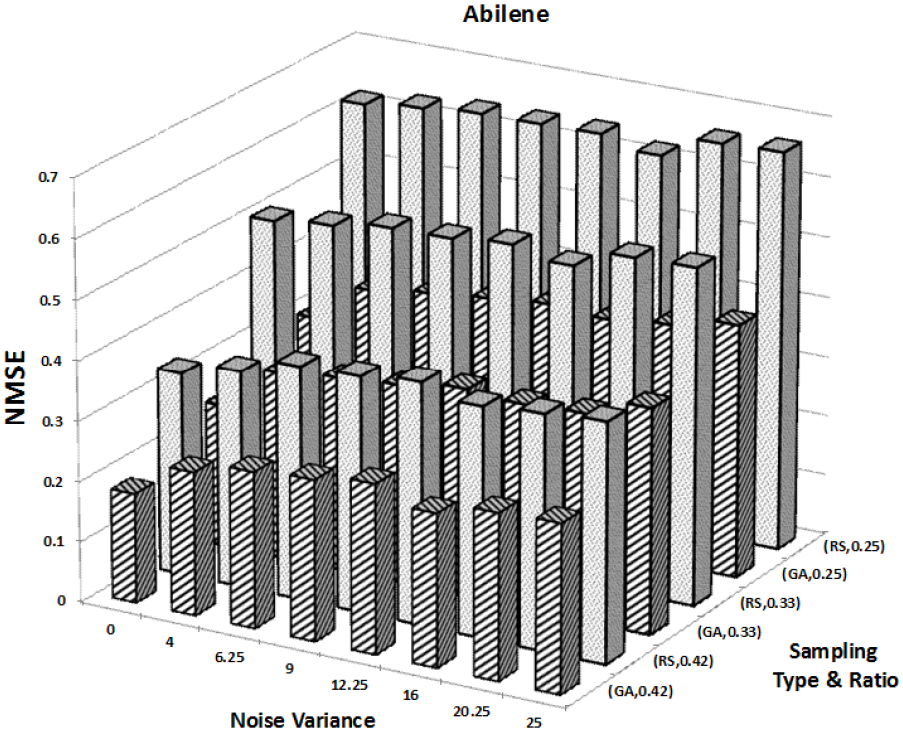
\includegraphics[width=\linewidth]{AbileneDelayNoise1.png} \hfill
  \caption{{The $NMSE$ v.s. SR \& noise for Abilene.}} \label{fig:AbileneGADelayNoise}
\endminipage\hfill
\minipage{0.40\textwidth}
  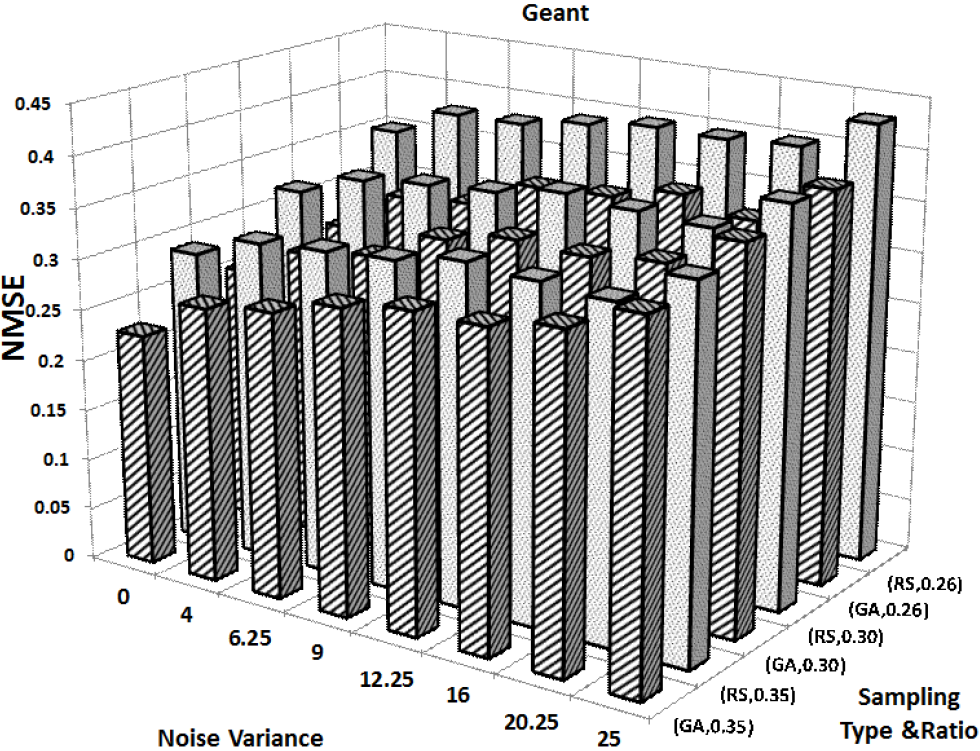
\includegraphics[width=\linewidth]{GeantDelayNoise1.png}
  \caption{{The $NMSE$ v.s. SR \& noise for Geant.}} \label{fig:GeantGADelayNoise}
\endminipage
\end{center}
\end{figure*}
%\begin{figure}
  %\begin{center}
    %{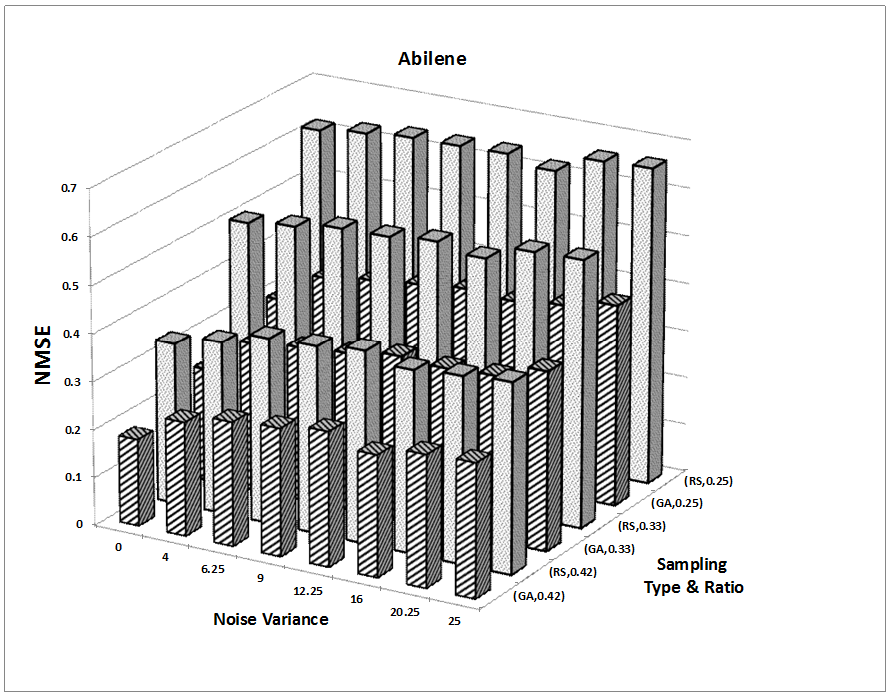
\includegraphics[keepaspectratio, width=0.49\textwidth]{AbileneDelayNoise.png}} % \\
    %{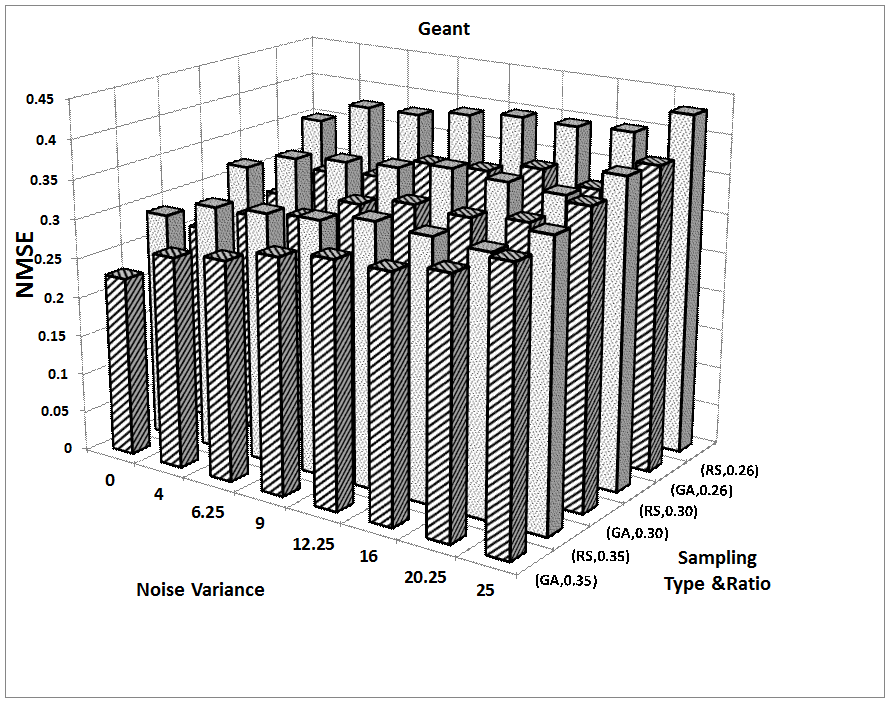
\includegraphics[keepaspectratio, width=0.49\textwidth]{GeantDelayNoise.png}}
  %\end{center}
  %\caption{{\footnotesize{The average $NMSE$ for different sampling types and ratios, and variances of queuing delay.}}}
  %\label{fig:AbileneGeantGADelayNoise}
%\end{figure}

\begin{figure}
  \begin{center}
    {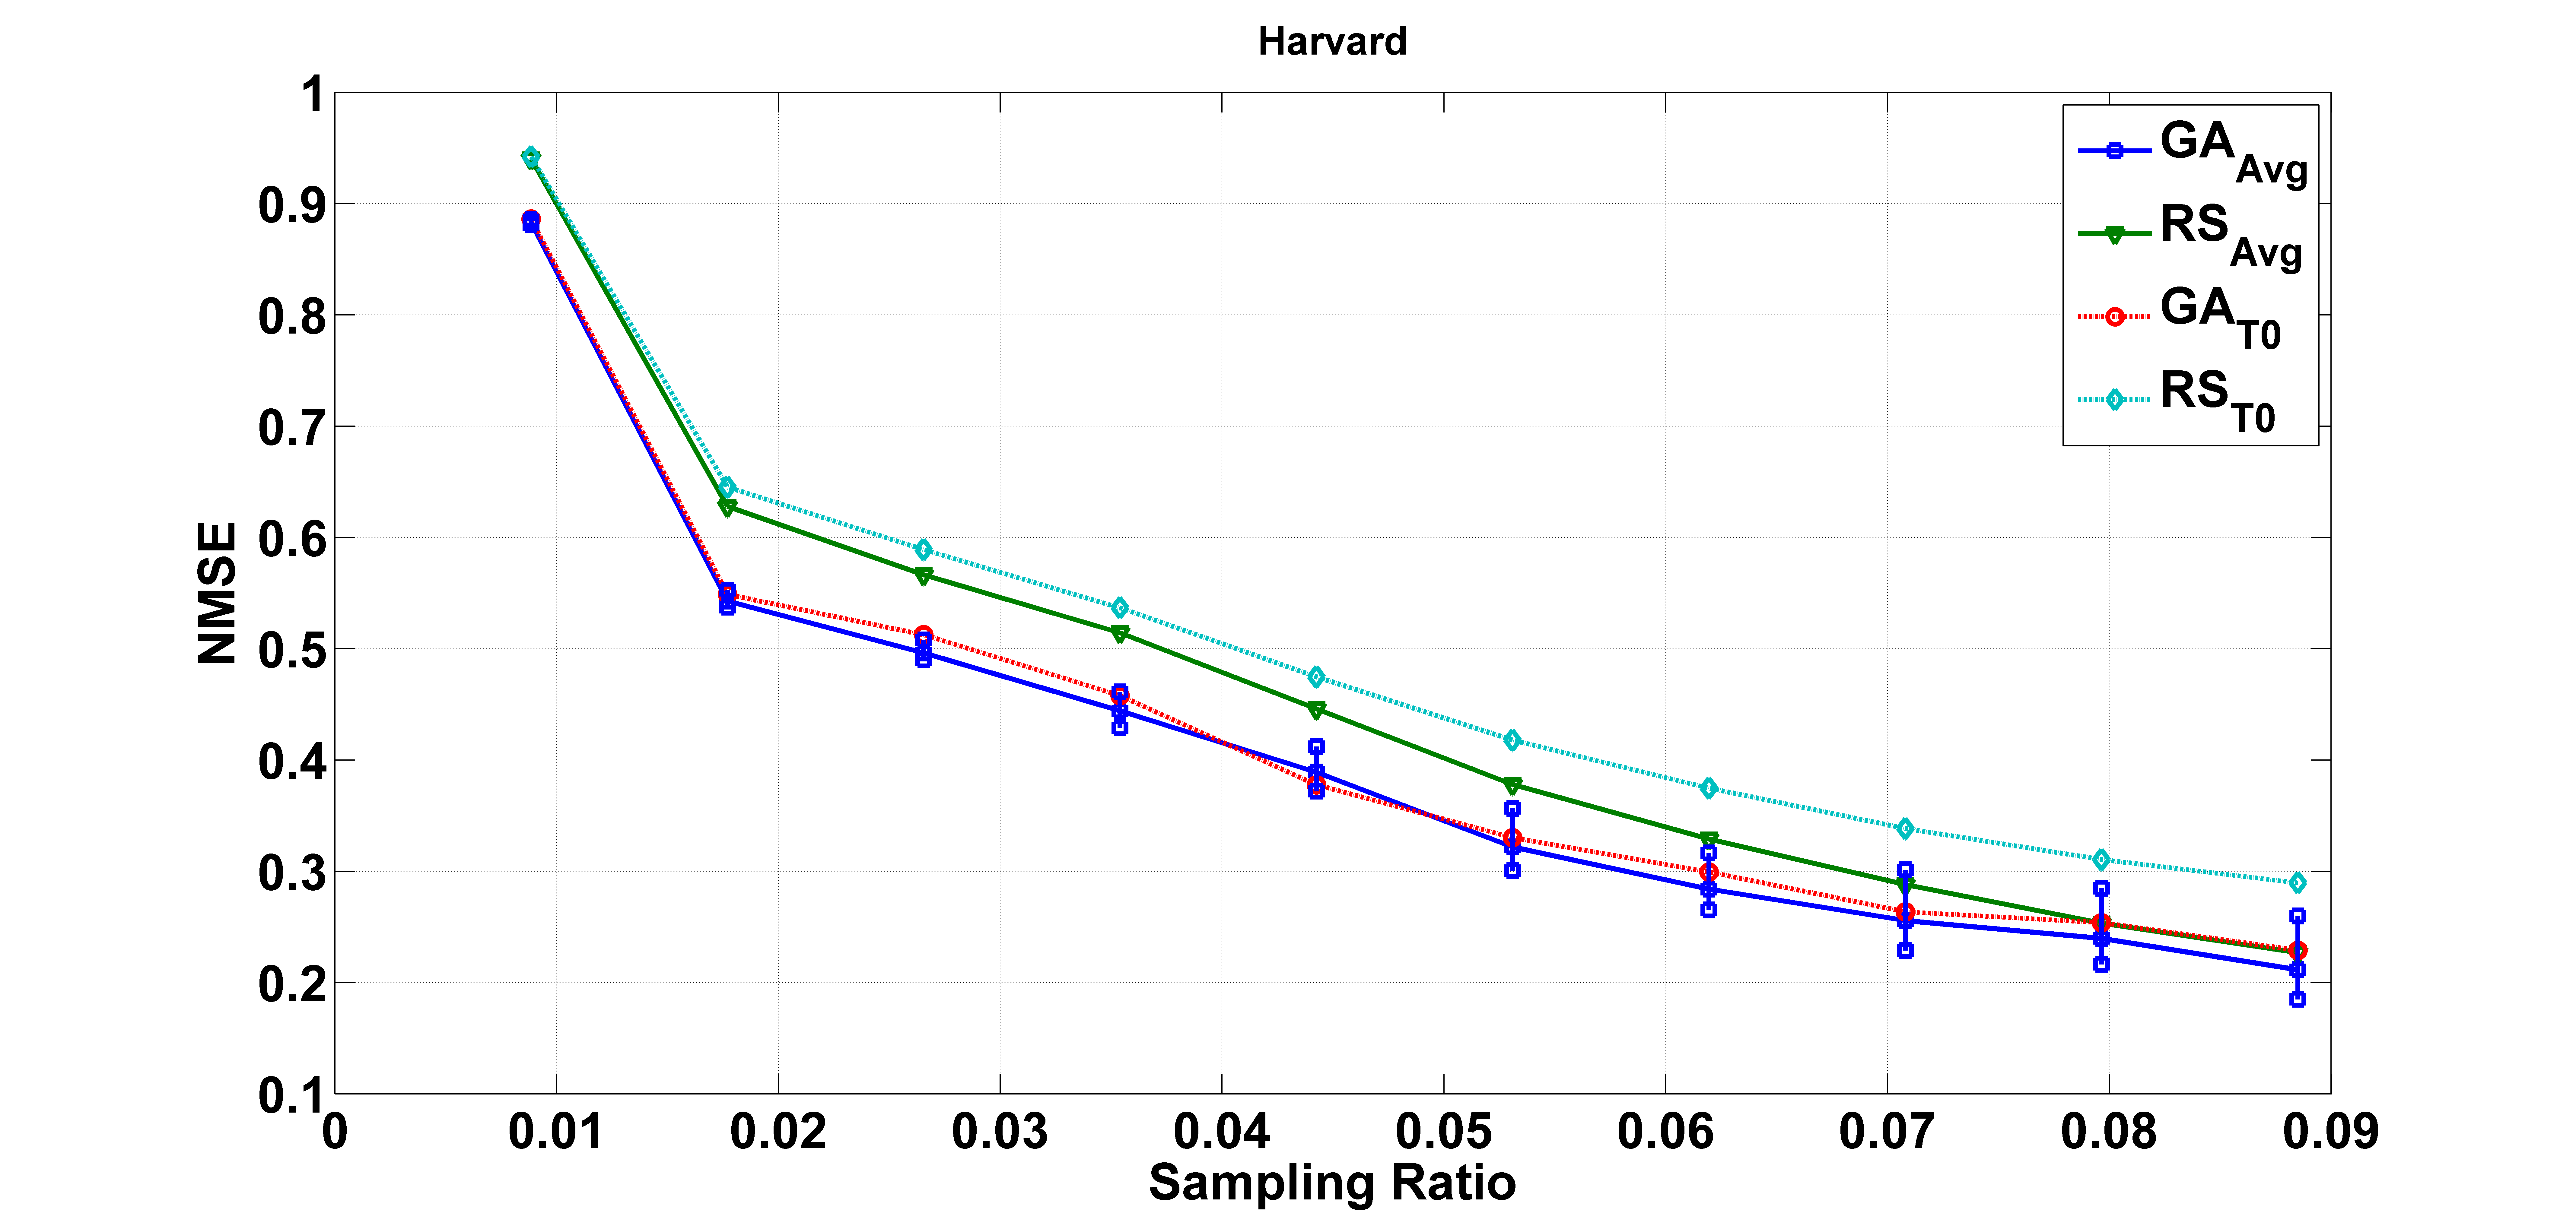
\includegraphics[keepaspectratio, width=0.49\textwidth]{HarvardGADelay.png}}
  \end{center}
  \caption{{{The $NMSE$ for Harvard network in different sampling ratios.}}}
  \label{fig:HarvardGADelayNoise}
\end{figure}

\begin{table}
	\centering
%  \footnotesize{
 \small{
 % \renewcommand{\tabcolsep}{0.05cm}
 % \renewcommand{\arraystretch}{1.0}
		\begin{tabular}{| c | c | c | c | c | c |}
		\hline
       $SR$           &    0.0088  &  0.0265  &  0.0442  &  0.0619  &  0.0796  \\ \hline
      $P^{d}_{CP}$    &    0.8077  &  0.9135  &  0.9306  &  0.9499  &  0.9566  \\ \hline
      $P^{fa}_{CP}$   &    0.4749  &  0.2412  &  0.1661  &  0.1263  &  0.1032  \\ \hline
    \end{tabular}
	% \caption{\scriptsize{The average of $P^{d}_{CP}$ and $P^{fa}_{CP}$ for Harvard network in different sampling ratios.}}
	\caption{{Average $P^{d}_{CP}$ and $P^{fa}_{CP}$ for Harvard network.}}
	\label{tab:PdfaHarvard}
}
\end{table}

\subsection{Per-Flow Size Estimation using SNIPER}
Figure \ref{fig:AbileneGeantGATMC} shows the performance of the SNIPER in the estimation of per-flow sizes on both Abilene and Geant networks using real traffic traces (see Table \ref{tab:DataSetProp}) where the MC technique is the SRSVD-base as in \cite{Roughan:2012}. Again, it is clear that by the optimal design of network measurement probes or equivalently the observation matrix, the performance of the matrix completion is improved, particularly at low sampling ratios which indicates the hard resource constraint of TCAM entries as the main resource for per-flow size measurement. The better accuracy is obtained almost for all sampling ratios. Table \ref{tab:SNIPERPdPfaHH} also shows the average performance of the SNIPER framework in the reliable detection of heavy hitters under low sampling ratios.  
% Therefore, comparing with random sampling strategy, this table indicates the good capability of this framework in detection HHs even under low sampling ratios.
\begin{figure}
  \begin{center}
    {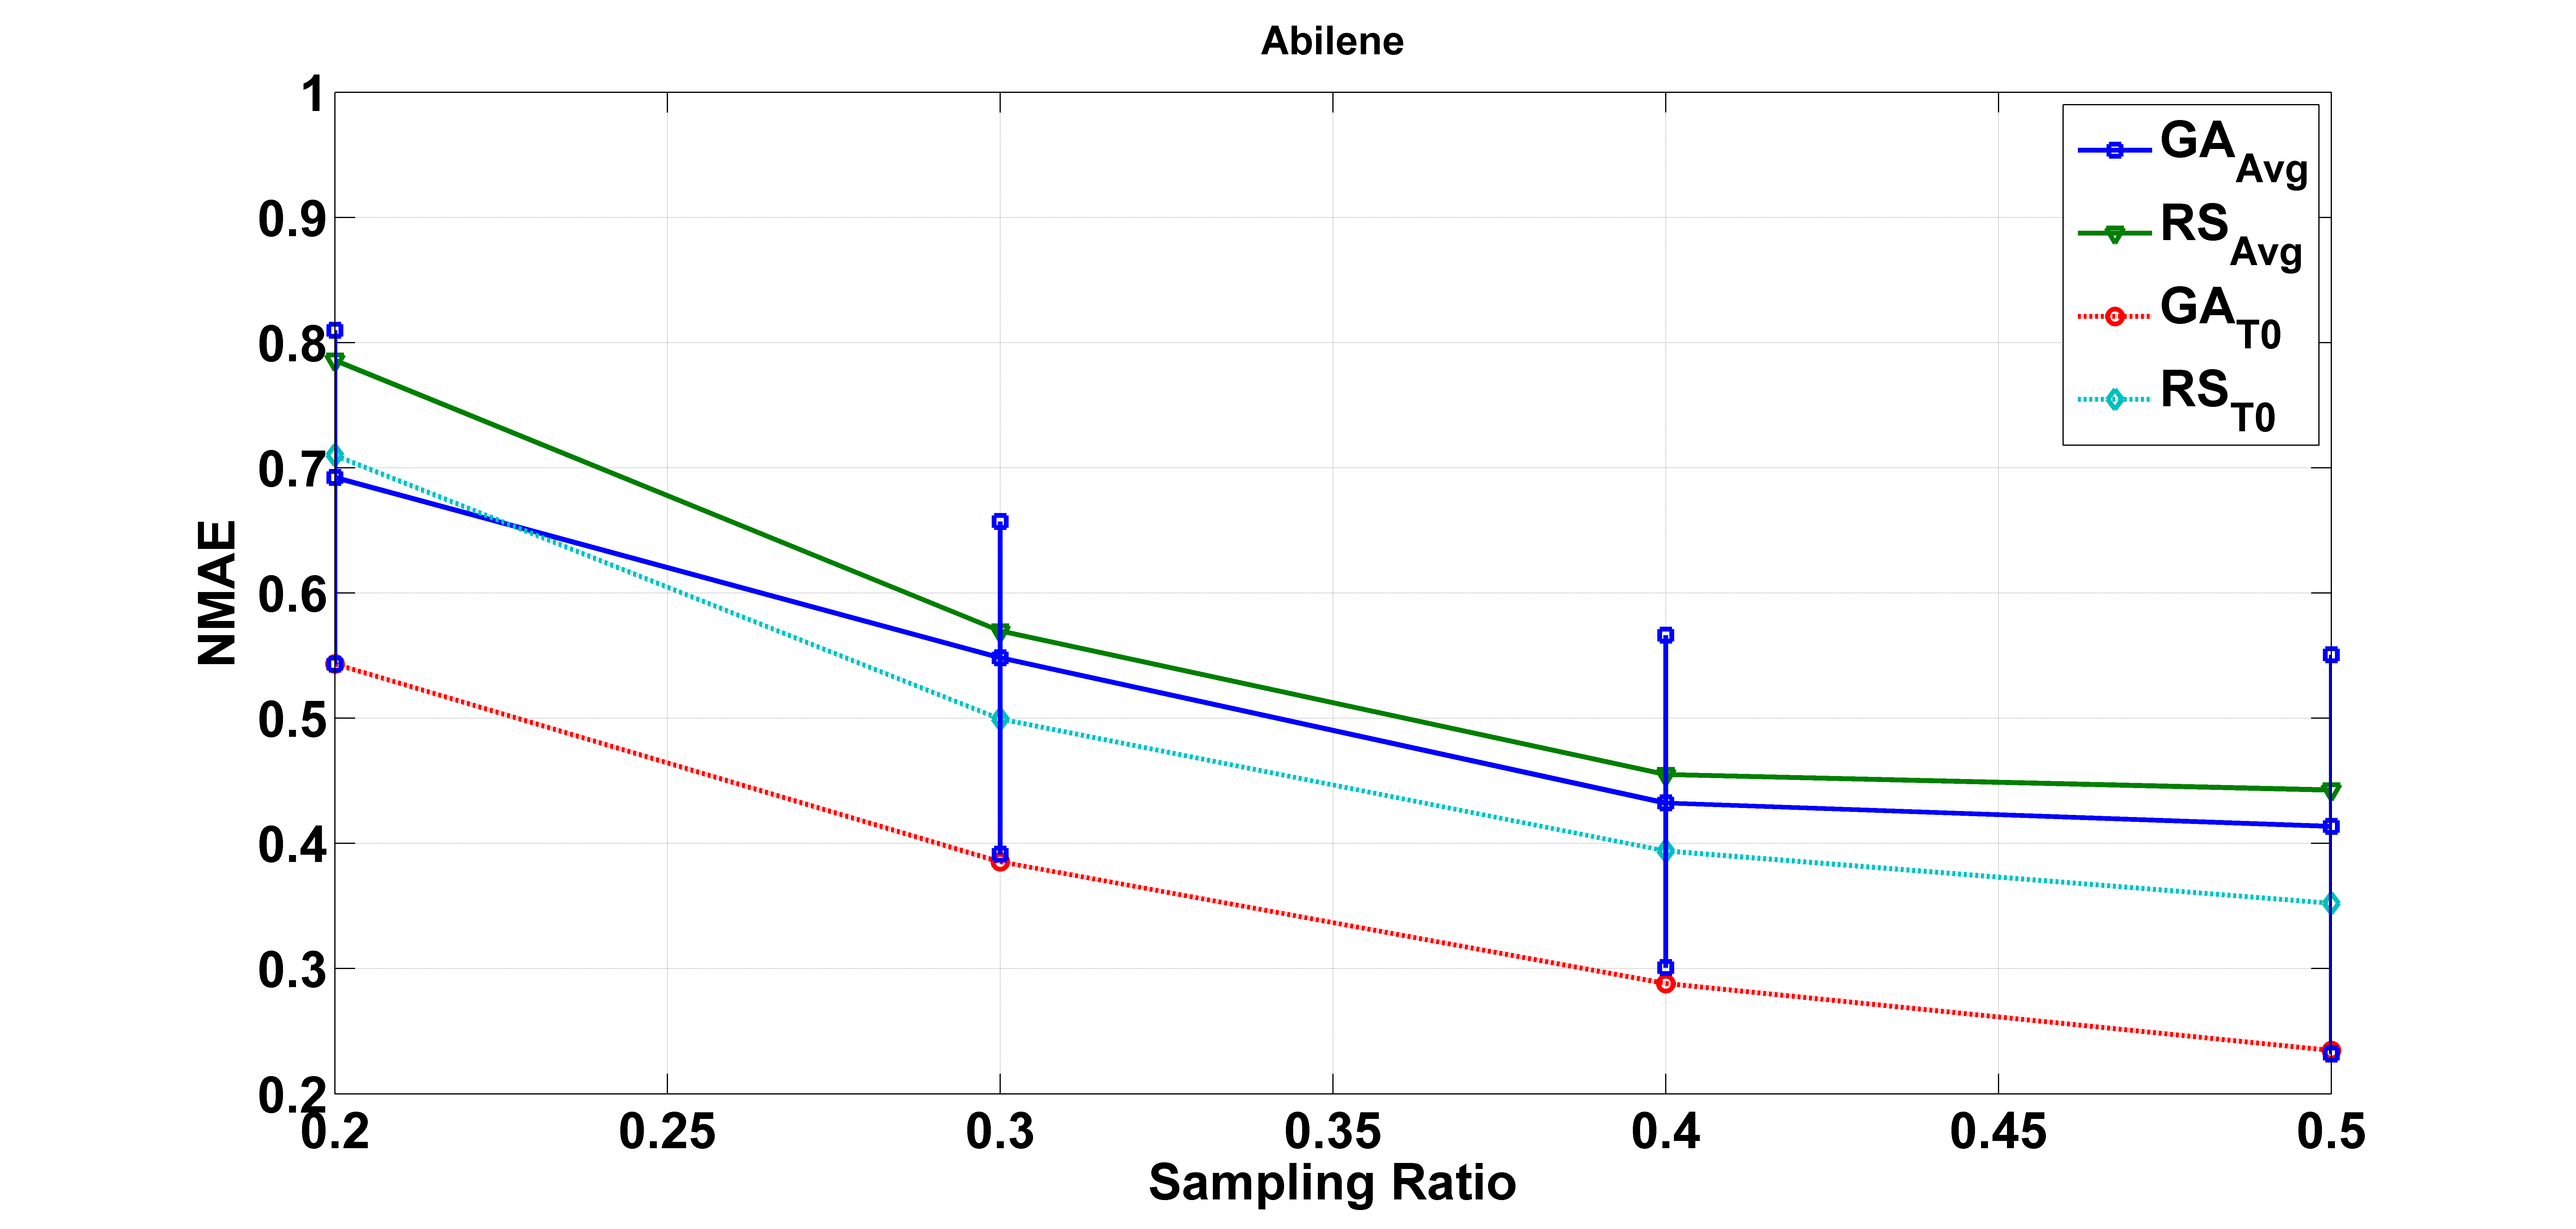
\includegraphics[keepaspectratio, width=0.49\textwidth]{AbileneGATMC.png}} \\
    {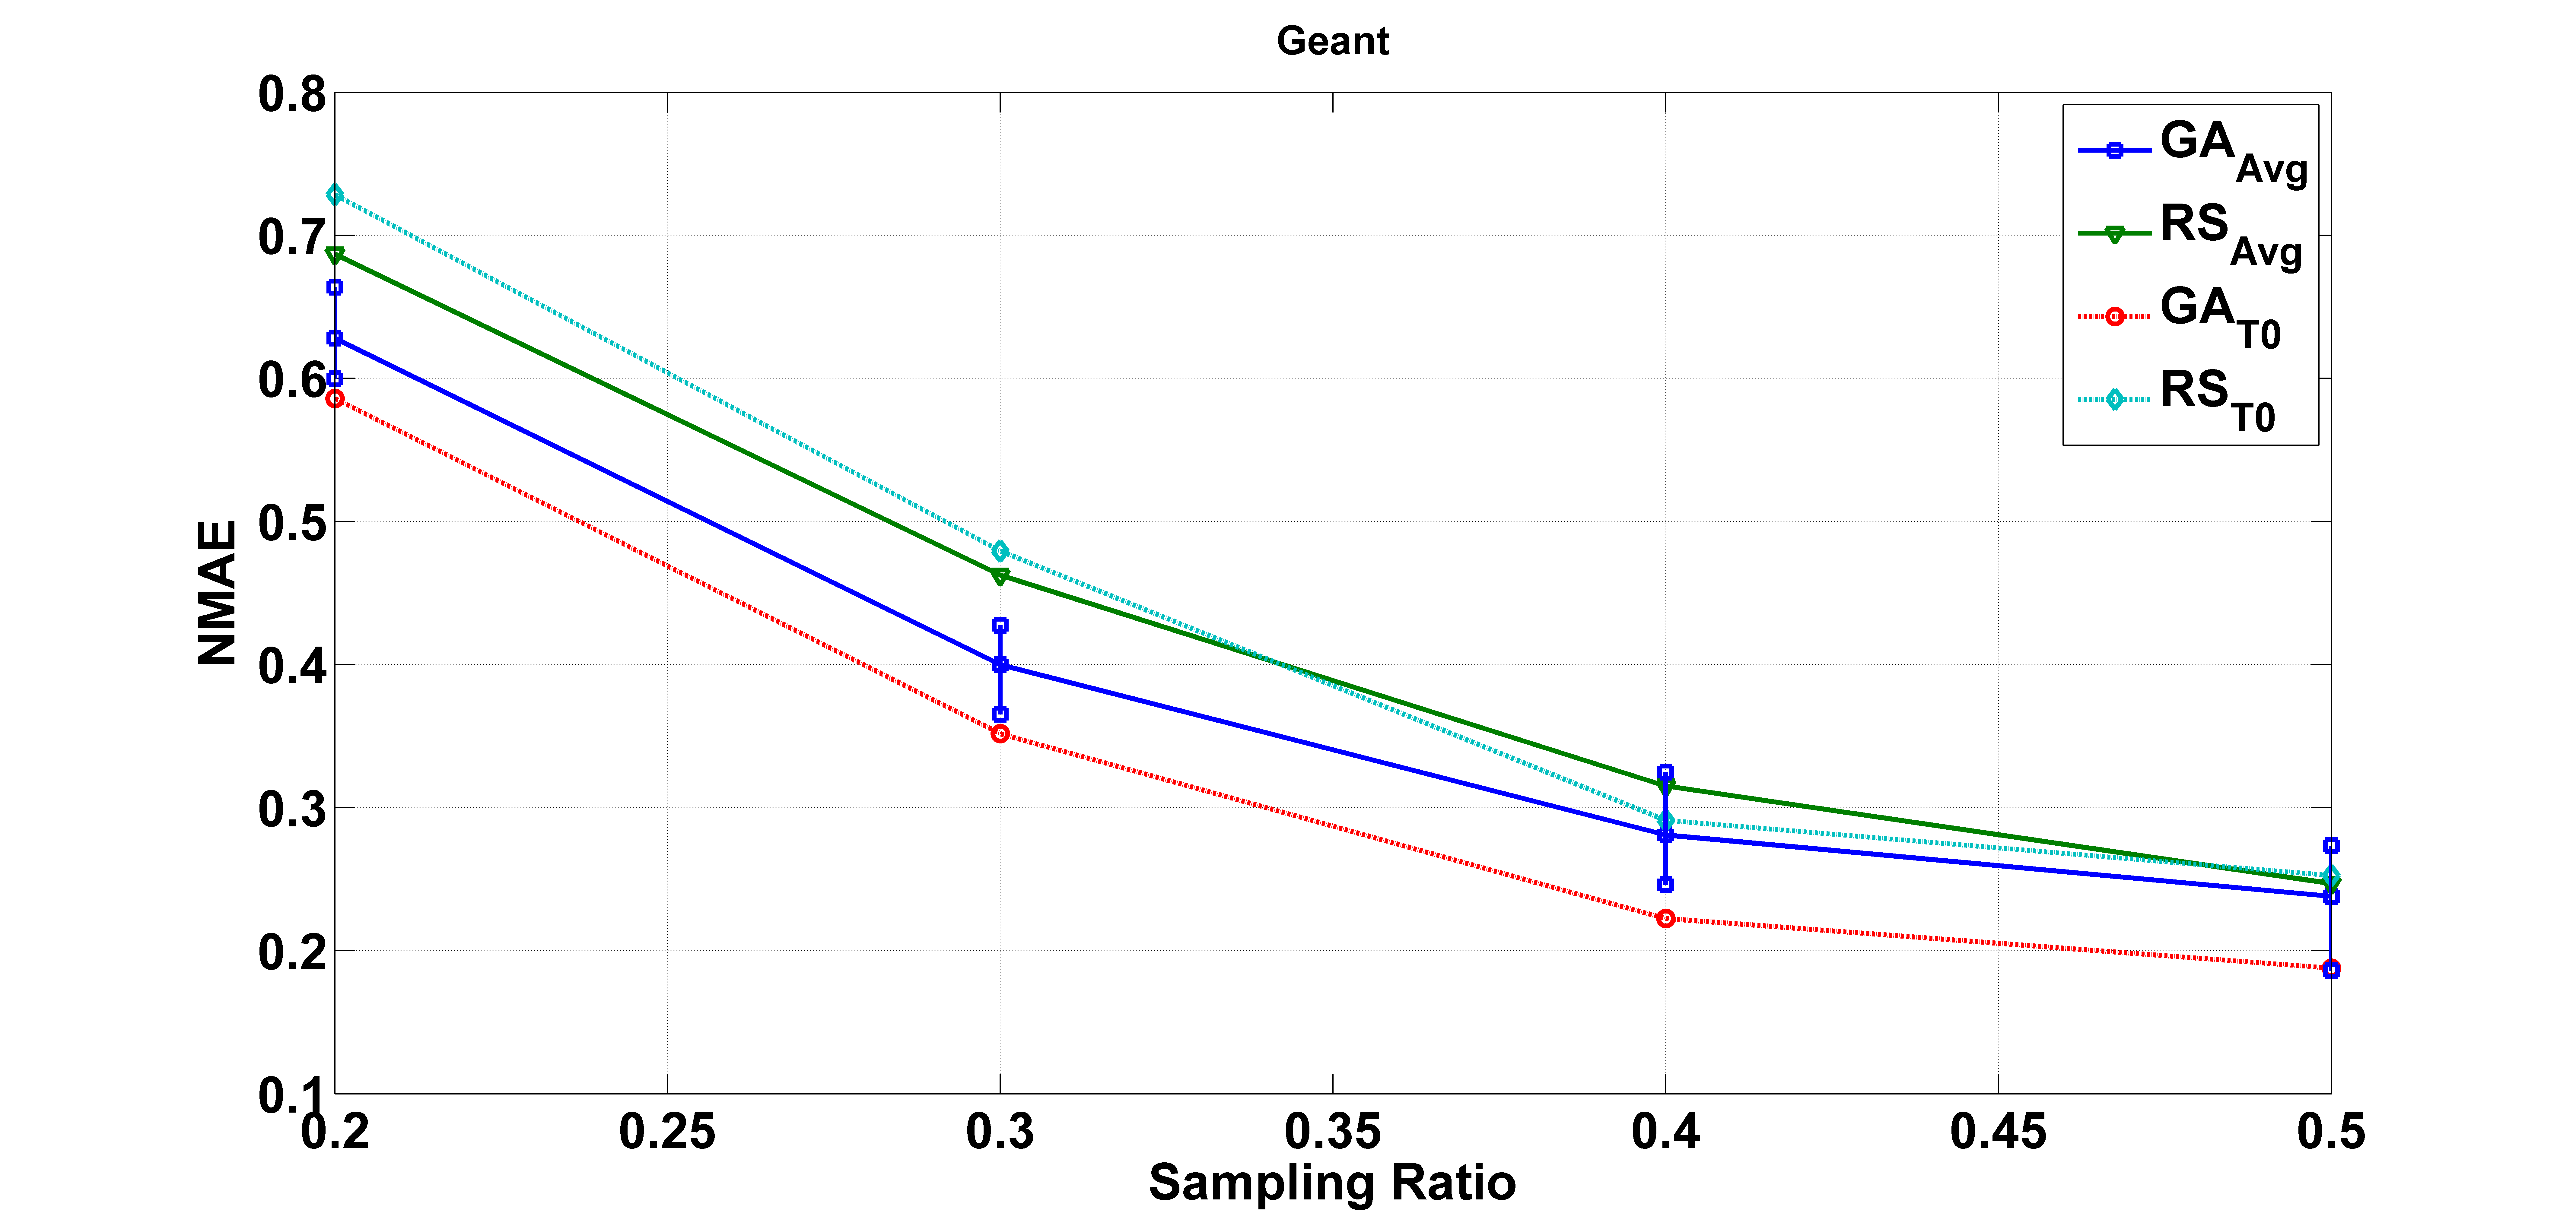
\includegraphics[keepaspectratio, width=0.49\textwidth]{GeantGATMC.png}}
  \end{center}
  \caption{{{$NMAE$ v.s. sampling ratios.}}}
  \label{fig:AbileneGeantGATMC}
\end{figure}

\begin{table}
	\centering
 \small{
 \renewcommand{\tabcolsep}{0.05cm}
 \renewcommand{\arraystretch}{1.0}
		\begin{tabular}{| c | c | c | c | c |}
		\hline
                                   & $SR=0.2$ & $SR=0.3$ & $SR=0.4$ & $SR=0.5$   \\ \hline
      $P^{d}_{HH}$ Abilene  (RS)   & 0.6256 & 0.7544 & 0.8426 & 0.8851 \\ \hline
      $P^{d}_{HH}$ Abilene  (GA)   & 0.6550 & 0.7693 & 0.8380 & 0.8901 \\ \hline
      $P^{fa}_{HH}$ Abilene   (RS) & 0.0353 & 0.0202 & 0.0144 & 0.0116 \\ \hline
      $P^{fa}_{HH}$ Abilene   (GA) & 0.0325 & 0.0192 & 0.0142 & 0.0119 \\ \hline
      $P^{d}_{HH}$ Geant   (RS)    & 0.7606 & 0.8935 & 0.9354 & 0.9489 \\ \hline
      $P^{d}_{HH}$ Geant   (GA)    & 0.7804 & 0.9096 & 0.9375 & 0.9502 \\ \hline
      $P^{fa}_{HH}$ Geant  (RS)    & 0.0106 & 0.0061 & 0.0043 & 0.0035 \\ \hline
      $P^{fa}_{HH}$ Geant  (GA)    & 0.0095 & 0.0058 & 0.0041 & 0.0034 \\ \hline
    \end{tabular}
%%%     \newline
%%% \vspace*{0.15cm}
%%% \newline
%		\begin{tabular}{| c | c | c | c | c |}
%		\hline
%                                   & $SR=0.2$ & $SR=0.3$ & $SR=0.4$ & $SR=0.5$   \\ \hline
%      $P^{d}_{HH}$ Geant   (RS)  \hspace{0.15cm}  & 0.7606 & 0.8935 & 0.9354 & 0.9489 \\ \hline
%      $P^{d}_{HH}$ Geant   (GA)  \hspace{0.15cm}  & 0.7804 & 0.9096 & 0.9375 & 0.9502 \\ \hline
%      $P^{fa}_{HH}$ Geant  (RS)  \hspace{0.15cm}  & 0.0106 & 0.0061 & 0.0043 & 0.0035 \\ \hline
%      $P^{fa}_{HH}$ Geant  (GA)  \hspace{0.15cm}  & 0.0095 & 0.0058 & 0.0041 & 0.0034 \\ \hline
%    \end{tabular}
  	\caption{{Comparing the average $P^{d}_{HH}$ and $P^{fa}_{HH}$ between RS and GA sampling and for Abilene and Geant networks where $\theta=0.05 C_{l}$ and $\theta=0.1 C_{l}$, respectively.}}
	\label{tab:SNIPERPdPfaHH}
}
\end{table}
%\begin{table}
%	\centering
% \small{
% \renewcommand{\tabcolsep}{0.05cm}
% \renewcommand{\arraystretch}{1.0}
%		\begin{tabular}{| c | c | c | c | c |}
%		\hline
%                              & $SR=0.2$ & $SR=0.3$ & $SR=0.4$ & $SR=0.5$   \\ \hline
%      $P^{d}_{HH}$ (Abilene)    & 0.6550   & 0.7693   & 0.8380   & 0.8851 \\ \hline
%      $P^{fa}_{HH}$ (Abilene)   & 0.0325   & 0.0192   & 0.0142   & 0.0119 \\ \hline
%      $P^{d}_{HH}$ (Geant)      & 0.7804   & 0.9096   & 0.9375   & 0.9502 \\ \hline
%      $P^{fa}_{HH}$ (Geant)     & 0.0095   & 0.0058   & 0.0041   & 0.0034 \\ \hline
%    \end{tabular}
%	\caption{\scriptsize{The average $P^{d}_{HH}$ and $P^{fa}_{HH}$ using GA for Abilene and Geant networks where $\theta=0.05 C_{l}$ and $\theta=0.1 C_{l}$, respectively.}}
%	\label{tab:SNIPERPdPfaHH}
%}
%\end{table}

%It is worth mentioning that, these results also have important implications in other applications such as recommended systems where, to reduce the number of measurements, we can intelligently ask particular customers to rate particular products which leads to the best estimate of all or sub-set of unknowns of interest. This is of particular importance, comparing with regular MC techniques which are based on the random measurements of the higher number of attributes of interest.

\subsection{Scalability of SNIPER}
As we have seen in the previous results, the SNIPER can improve the estimation accuracy under hard resource constraint regimes. To reduce the high computational complexity of the GA in designing the OOM in large-scale networks and increase the scalability of the SNIPER framework, here, we use the PSO evolutionary optimization algorithm which is much faster than the GA \cite{Talib:2009}\cite{Kachitvichyanuku:2012} and it can reduce the computational complexity and processing power of the SNIPER. Figure \ref{fig:AbileneGeantPSOTMC} shows the performance of SNIPER for per-flow size estimation, representing the fact that in low sampling rates the intelligent design of the observation matrix using PSO algorithm results in a better estimation accuracy. The reduction in the computational complexity using the PSO algorithm is quantified using the notion of Processing Gain ($PG$) defined as $PG := 100 \times \frac{PT_{GA}-PT_{PSO}}{PT_{GA}}$ (in \%) where $PT_{GA}$ and $PT_{PSO}$ respectively denote the processing times for running GA and PSO algorithms. The processing gains for Abilene and Geant networks are $PG$=56\% and $PG$=65\%, respectively. 
%************* explain the norm in appendix  and say that it is under investigation ******************8
%In Appendix A we propose another method to address the scalability 
%\begin{equation}\label{DefPG}
%\small{
%\begin{aligned}
%PG = 100 \times \frac{PT_{GA}-PT_{PSO}}{PT_{GA}}
%\end{aligned}
%}
%\end{equation}
\begin{figure}
  \begin{center}
    {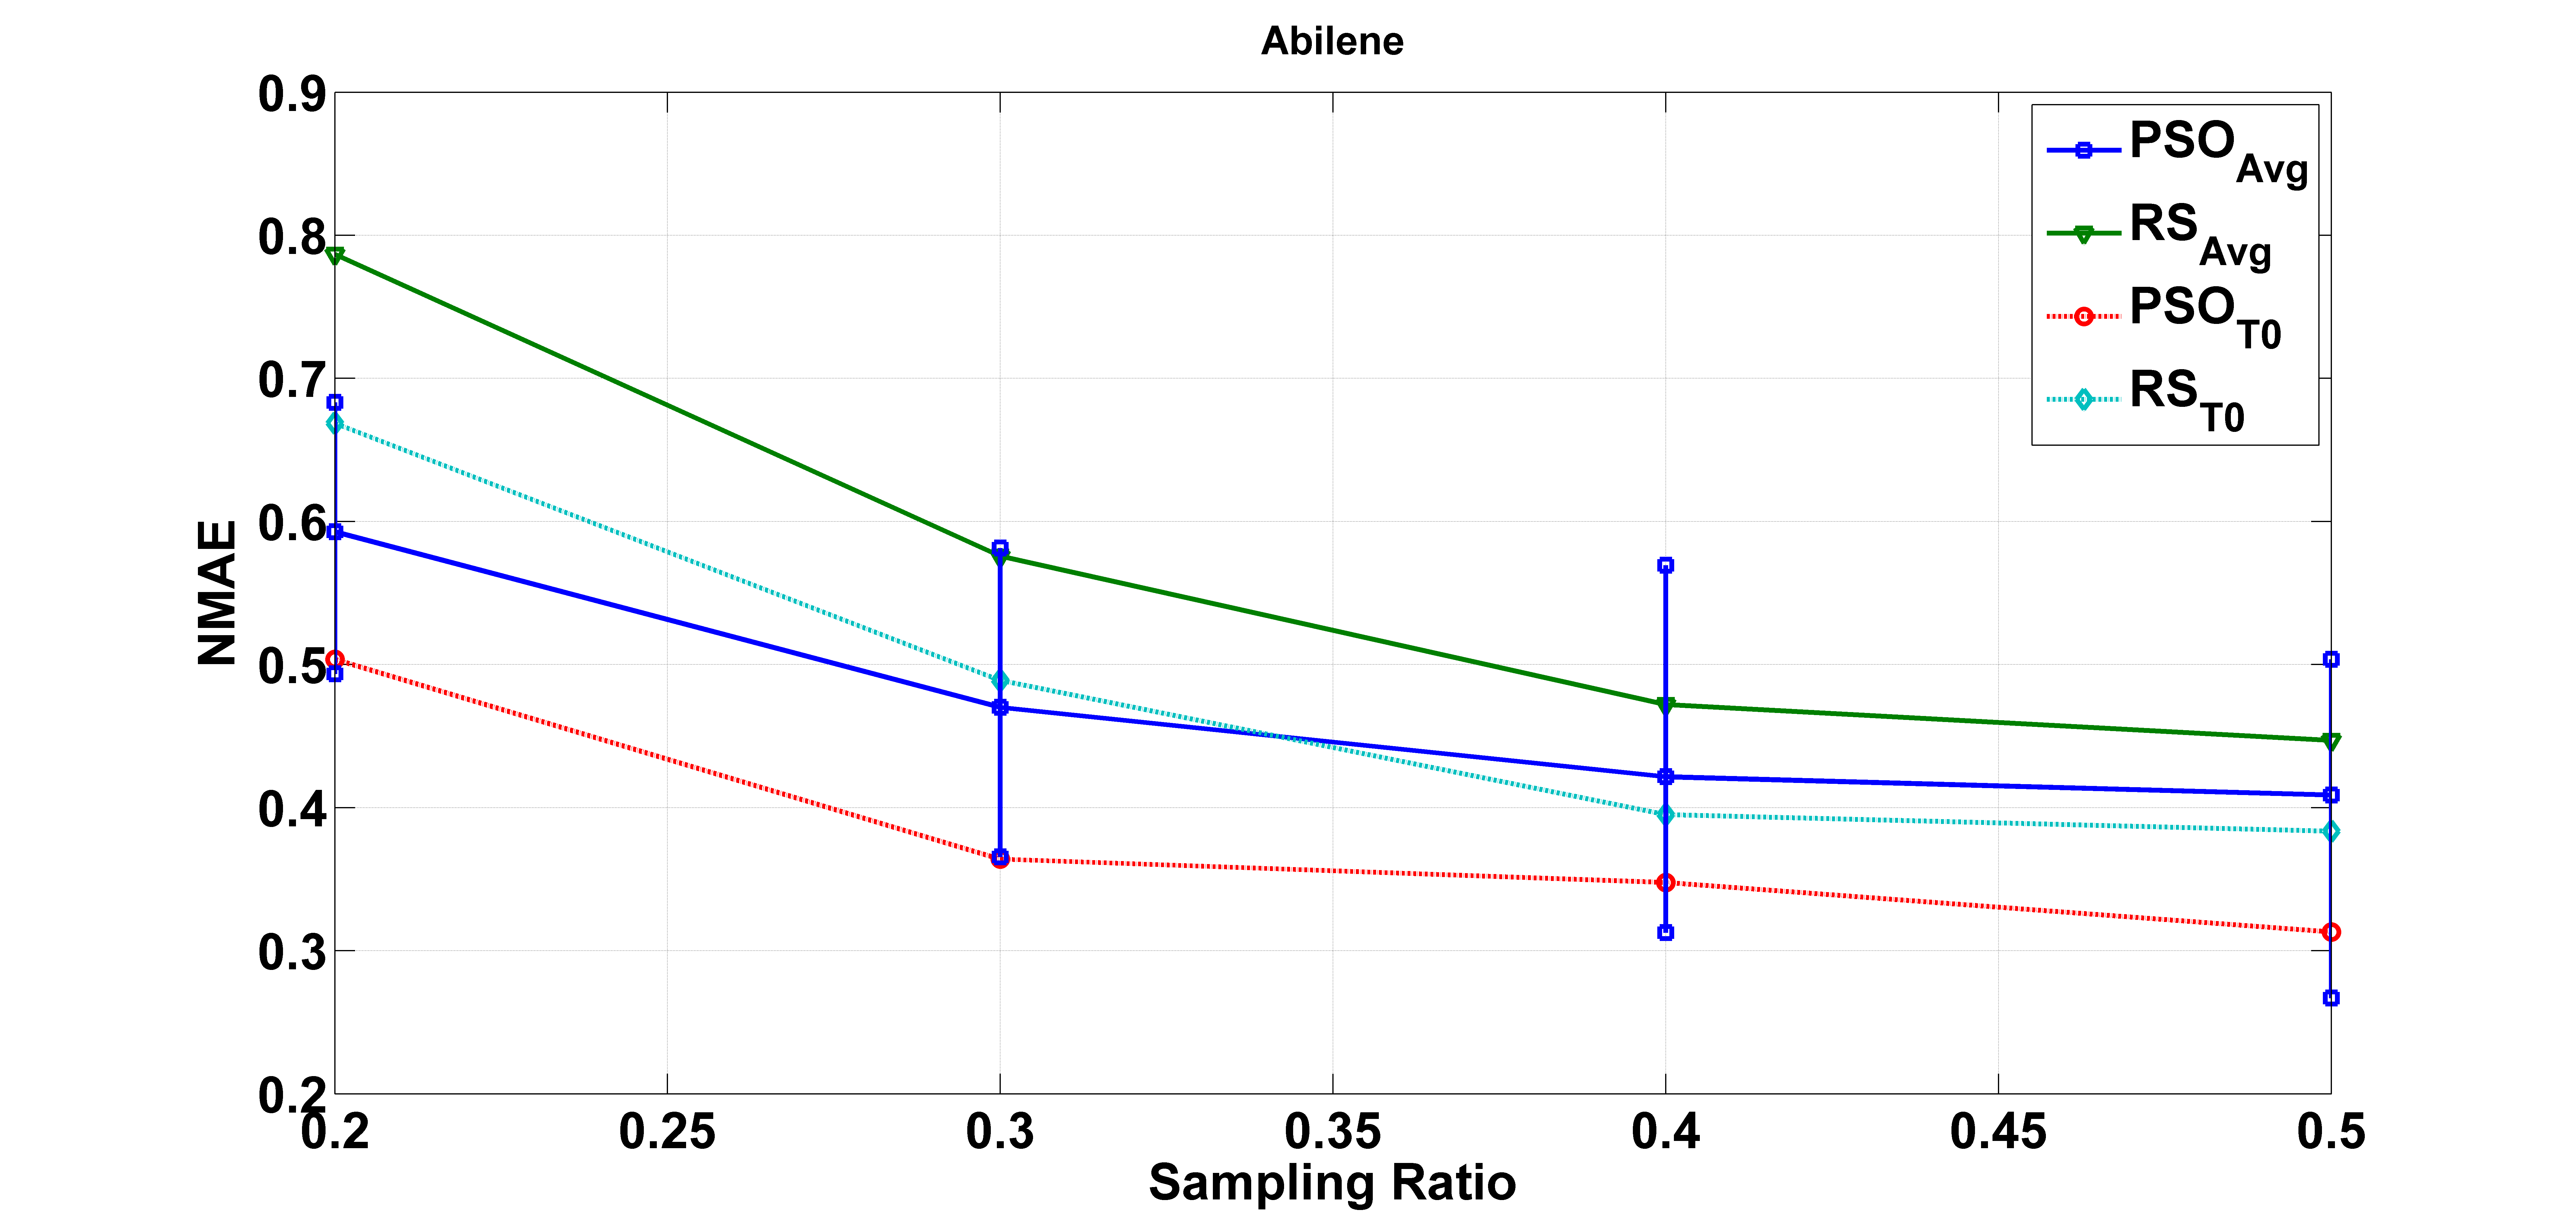
\includegraphics[keepaspectratio, width=0.49\textwidth]{AbilenePSOTMC.png}} \\
    {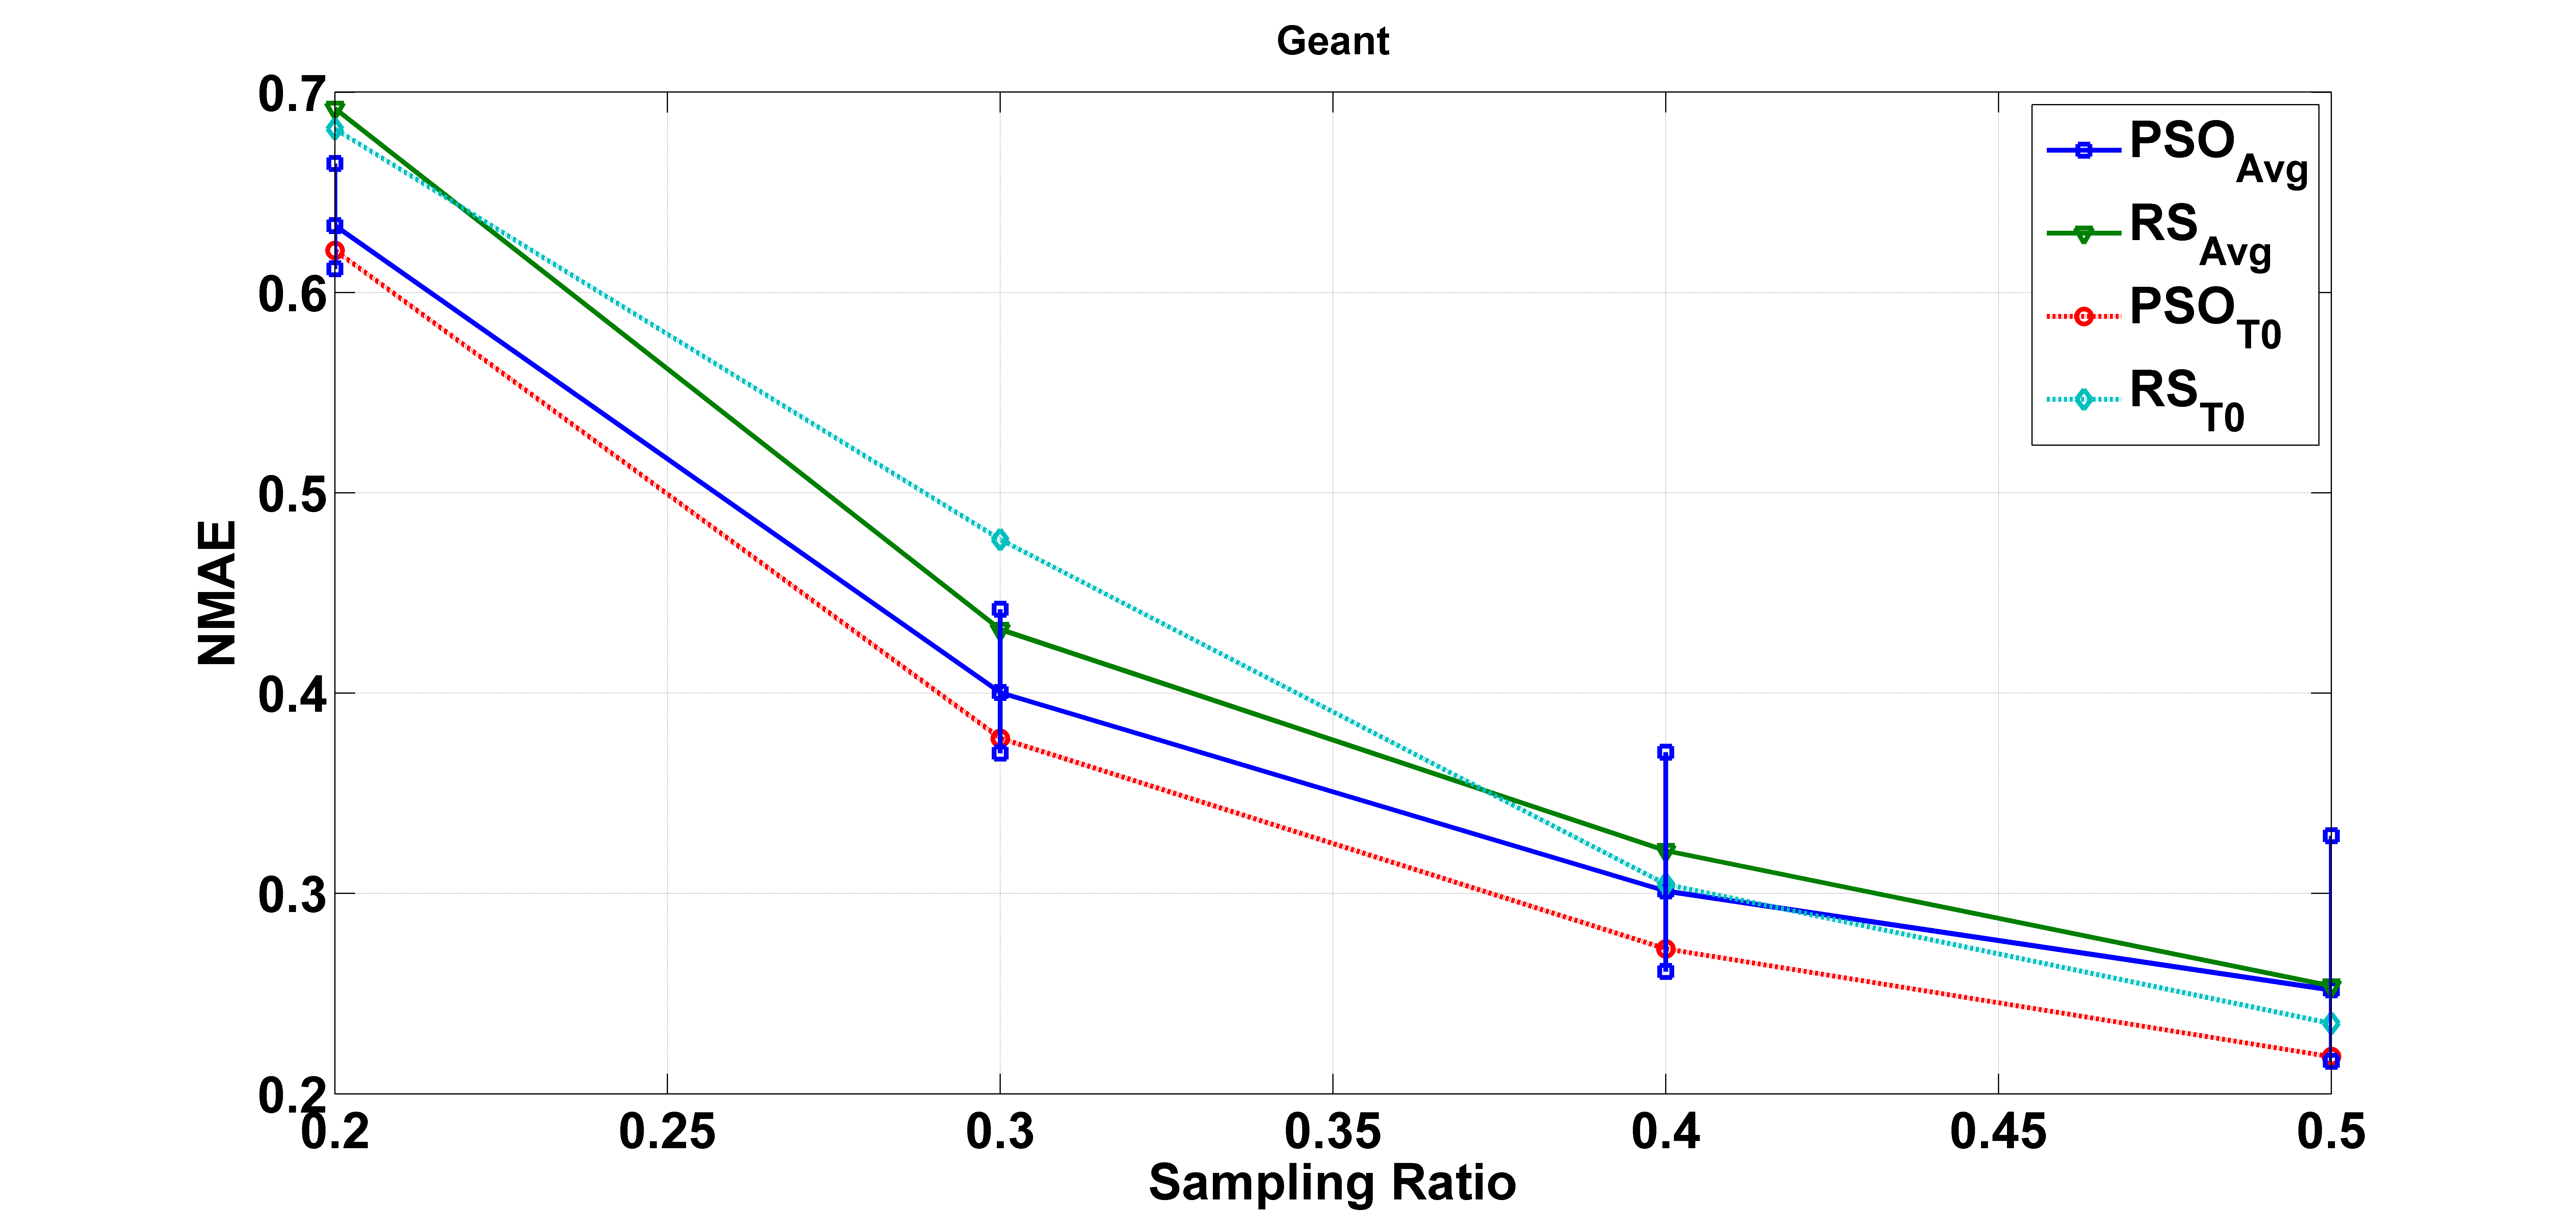
\includegraphics[keepaspectratio, width=0.49\textwidth]{GeantPSOTMC.png}}
  \end{center}
  \caption{{{$NMAE$ v.s. sampling ratios.}}}
  \label{fig:AbileneGeantPSOTMC}
\end{figure}
%In addition, instead of minimizing the ultimate estimation accuracy (e.g. represented by $NMAE$), the norm of the observation matrix $\Omega$  is minimized where the norm of a matrix is defined as the maximum singular value of the matrix and denoted by $sigma_{1}(\Omega)$. Note that, the norm of the observation matrix is strongly correlated with $NMAE$; this fact has been justified in Figure \ref{fig:NMAENormCorrFig} and Table \ref{tab:NMAENormCorrTab}. Also, Tables \ref{tab:FitFuncCmp1} and \ref{tab:FitFuncCmp2} shows the NMAE and the processing gains (indicated by the Time Gain) achieved by minimizing the norm of the observation matrix using both GA and PSO algorithms. Due to some inconsistency in  Table \ref{tab:FitFuncCmp1} this paragraph and its results are removed; in fact, we can conclude that to achieve a better accuracy the ultimate performance metric must be optimized.
%\begin{table}
%	\centering
% \footnotesize{
% \renewcommand{\tabcolsep}{0.05cm}
% \renewcommand{\arraystretch}{1.0}
%		\begin{tabular}{| c | c | c | c | c | c | c | c |}
%		\hline
%       Net./Prm. & $SR$ & $RS_{T_{0}}$ & $GA_{T_{0}}$ & $PSO_{T_{0}}$ & $RS^{\sigma}_{T_{0}}$ & $GA^{\sigma}_{T_{0}}$ & $PSO^{\sigma}_{T_{0}}$  \\ \hline
%      Abilene    & 0.3 & 0.499312 & 0.364073 & 0.387655 & 0.498732 & 0.503375 & 0.480801 \\ \hline
%      GEANT      & 0.2 & 0.728394 & 0.55408 & 0.60432 & 0.722275 & 0.679437 & 0.684696 \\ \hline
%    \end{tabular}
%    \newline
%\vspace*{0.15cm}
%\newline
%		\begin{tabular}{| c | c | c | c | c | c | c | c |}
%		\hline
%       Net./Prm. & $SR$ & $RS_{Avg}$ & $GA_{Avg}$ & $PSO_{Avg}$ & $RS^{\sigma}_{Avg}$ & $GA^{\sigma}_{Avg}$ & $PSO^{\sigma}_{Avg}$  \\ \hline
%      Abilene    & 0.3 & 0.569638 & 0.556108 & 0.494916 & 0.582961 & 0.546438 & 0.586098  \\ \hline
%      GEANT      & 0.2 & 0.686854 & 0.601478 & 0.644993 & 0.69442 & 0.664646 & 0.681144  \\ \hline
%    \end{tabular}
%	\caption{\scriptsize{NMAE comparison between different evolutionary fitness functions ($\sigma$ denotes norm function).}}
%	\label{tab:FitFuncCmp1}
%}
%\end{table}
%
%\begin{table}
%	\centering
% \footnotesize{
% \renewcommand{\tabcolsep}{0.05cm}
% \renewcommand{\arraystretch}{1.0}
%		\begin{tabular}{| c | c | c | c |}
%		\hline
%       Net./TimeGain & $SR$ & $Time Gain^{\sigma}_{GA}$ & $Time Gain^{sigma}_{PSO}$ \\ \hline
%      Abilene    & 0.3 & 0.937689 & 0.818912  \\ \hline
%      GEANT      & 0.2 & 0.884593 & 0.773611  \\ \hline
%    \end{tabular}
%	\caption{\scriptsize{Time Gain comparison between different evolutionary fitness functions ($\sigma$ denotes norm function).}}
%	\label{tab:FitFuncCmp2}
%}
%\end{table}
%\begin{figure}
%  \begin{center}
%    {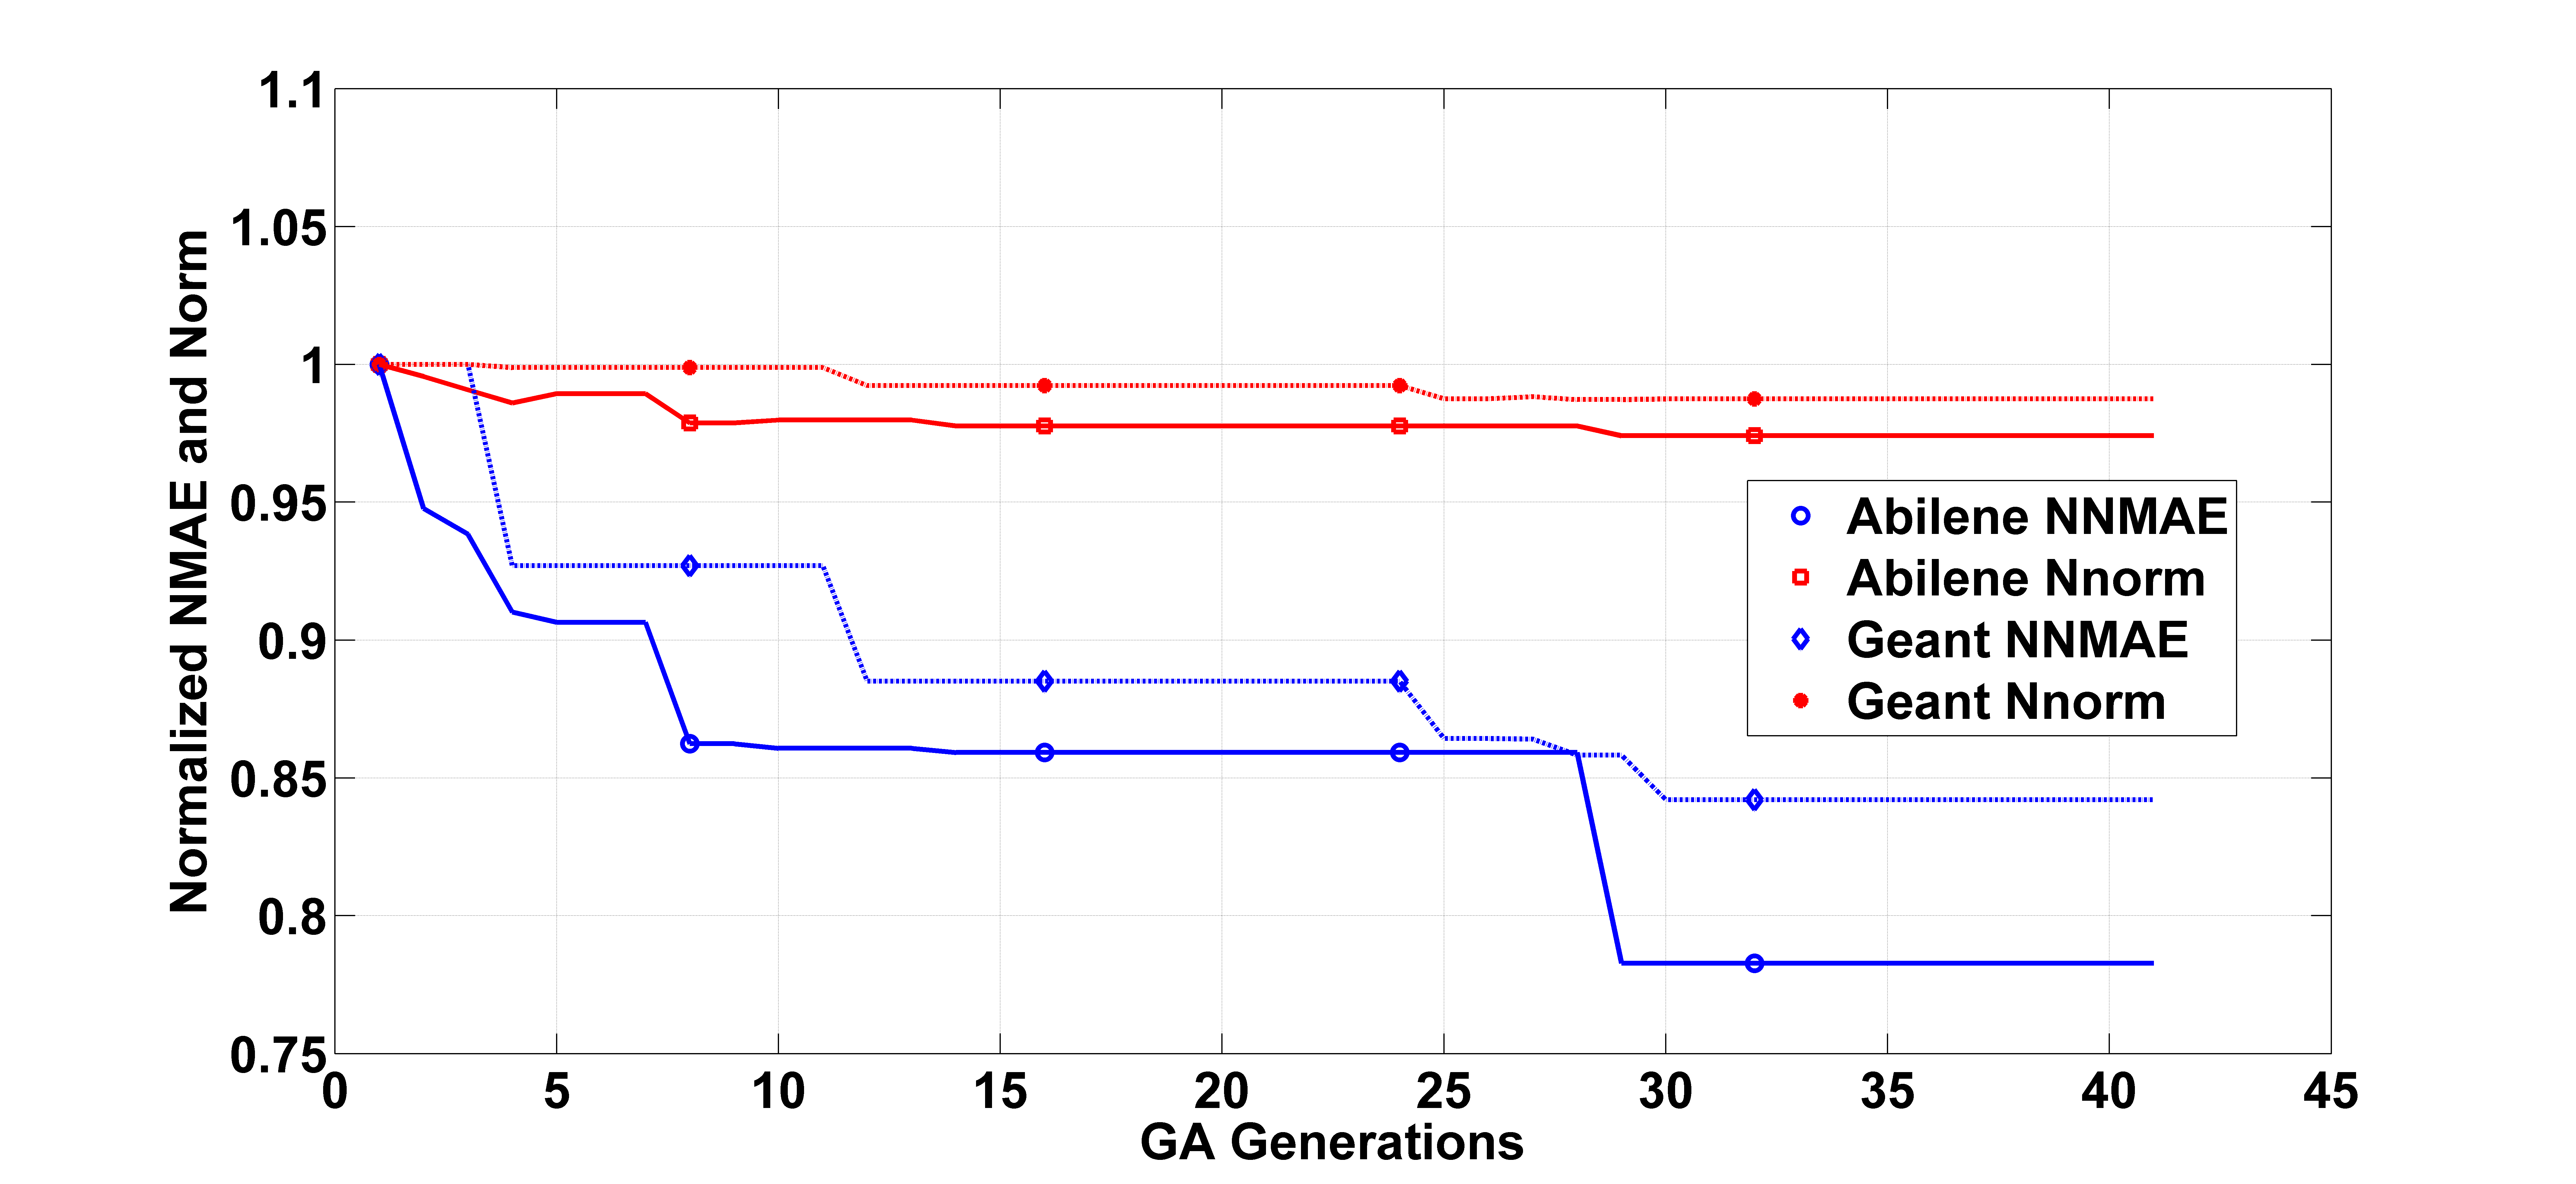
\includegraphics[keepaspectratio, width=0.49\textwidth]{AbileneGeantGAEvolution.png}}
%  \end{center}
%  \caption{{\footnotesize{The evolution of normalized $NMAE$ and norm in the GA.}}}
%  \label{fig:NMAENormCorrFig}
%\end{figure}
%
%\begin{table}
%	\centering
% \small{
% \renewcommand{\tabcolsep}{0.05cm}
% \renewcommand{\arraystretch}{1.0}
%		\begin{tabular}{| c | c | c | c | c |}
%		\hline
%                       & $SR=0.2$ & $SR=0.3$ & $SR=0.4$ & $SR=0.5$   \\ \hline
%      $\rho$ Abilene   & 0.9089 & 0.9640 & 0.7546 & 0.9698 \\ \hline
%      $\rho$ Geant     & 0.9337 & 0.8805 & 0.9617 & 0.8791 \\ \hline
%    \end{tabular}
%	\caption{\scriptsize{Correlation coefficient $\rho:=\frac{Cov(NMAE,\sigma_{1}(\Omega))}{\sqrt{Var(NMAE)Var(\sigma_{1}(\Omega))}}$ between NMAE and the norm of the observation matrix}}
%	\label{tab:NMAENormCorrTab}
%}
%\end{table}

\subsection{Deployability of SNIPER in Dynamic Environments}
In the case of supervised learning, the SNIPER framework computes the optimal sampling matrix using the training data, available in the initial learning stage. The training data set can be obtained by directly measuring the required IAI in the beginning or by using already available data sets (e.g. NetFlow records in the case of TM completion). Under hard constraint of network measurement resources, to effectively apply the SNIPER framework in dynamic environments, it is important to: 1) decrease the dependency of the SNIPER framework on the initial training data set, and 2) adaptively update the OOM designed in the initial stage based on the most current behavior of the network under study. Accordingly, here, we propose a new algorithm that can be effectively utilized for network measurement purposes in the SNIPER framework. 

In this algorithm, first, we determine the initial sampling ratio (indicated by $s_{0}$) and over the initial period we use SDN flexibility to randomly measure a sub-set of IAI to form a matrix with size $n \times T_{0}$. Then, we apply the appropriate matrix completion on this matrix of IAI to estimate unknown IAI and form our new training data set. Then we apply the evolutionary optimization algorithm (e.g. GA) on this new training data set to compute the OOM. By applying the MC algorithm using this OOM we can estimate all unknown IAI. Since the largest IAI are potentially the most informative ones for increasing the estimation accuracy \cite{IF14iSTAMP:2014}, to adaptively update the OOM for use in the next measurement epoch, we also choose a fraction of largest estimated IAI (indicated by $k_{0}$) to be measured directly. That is, after learning epoch where the OOM is designed using the new training data set, we modify this optimal measurement matrix by adding $k_{0}$ direct measurements which are indicated by the largest estimated IAI in the previous epoch. 

%In this algorithm, to reduce the dependency of the SNIPER framework on the initial training data set, first, we determine the initial sampling ratio (indicated by $s_{0}$) and randomly measure a sub-set of IAI to form a matrix with size $n \times T_{0}$. Then, we apply the appropriate matrix completion on this matrix of IAI to estimate unknown IAI and form our new training data set. Then we apply the evolutionary optimization algorithm (e.g. GA) on this new training data set to compute the optimal observation matrix. By applying the MC algorithm using this optimal observation matrix we can estimate all unknown IAI. Since the largest IAI are potentially the most informative ones for increasing the estimation accuracy \cite{IF14iSTAMP:2014}, to adaptively update the optimal observation matrix for use in the next measurement epoch, we also choose a small number of largest estimated IAI (indicated by $k_{0}$) to be measured directly. That is, after learning epoch where the optimal observation matrix is designed using the new training data set, we modify this optimal measurement matrix by adding $k_{0}$ direct measurements which are indicated by the largest estimated IAI in the previous epoch. 
% In fact, as it has been shown in \cite{IF14iSTAMP:2014}, largest IAI (i.e. flows) are the most informative IAI for network inference algorithms. 

Table \ref{tab:NMAEDGA} shows the performance of this algorithm where the genetic algorithm is used to design the OOM. Here, the notions of DGA and DRS are respectively used to denote Dynamic GA and Dynamic RS indicating the case where initial observation matrix is adaptively updated. It is clear that, under hard resource constraint regime, that is at low sampling ratio $SR$=0.2, the DGA is able to provide more accurate estimates of estimated flows on both Abilene and Geant networks. Also, there is a trade-off between the performance and parameters $s_{0}$, which controls the dependency of the SNIPER framework on the training data set, and $k_{0}$ which determines the number of new measurements to update the OOM matrix. Table \ref{tab:PdPfaDGA} also show that this algorithm can reliably detect heavy hitters under hard resource constraint of TCAM entries as the main resource used for traffic measurement in SDN switches.

%The OEOA can be used by the SNIPER framework to improve its performance in dynamic environments where the characteristics of the IAI varies and online measurements are needed to capture the most current behavior of the network under study. Assuming a pre-determined sampling ratio, the OEOA is performed in the following steps.
%
%It starts by the random measurement of a sub-set of the attribute of interests (denoted by $\Omega$). Then, it applies the matrix completion technique to estimate unobserved IAI in the set $\bar{\Omega}$. Next, it considers the estimates in the first step (in the set $\bar{\Omega}$) as measurements and apply the same MC technique to estimate the entries in the set $\Omega$ that we have already measured them, precisely. Now, the OEOA has the ability to evaluate the fitness value for each solution in the population
%
%\begin{table}
	%\centering
%%  \footnotesize{
 %\small{
 %% \renewcommand{\tabcolsep}{0.05cm}
 %% \renewcommand{\arraystretch}{1.0}
		%\begin{tabular}{| c | c | c | c | c | c | c |}
		%\hline
       %$SR$                                  &    $RS_{T_{0}}$  &  $GA_{T_{0}}$  &  $GA_{Avg}$  &  $RS_{Avg}$ &  $DRS_{Avg}$ &  $DGA_{Avg}$ \\ \hline
      %Abilene ($s_{0}$=0.5) &        &       &      &     &  &        \\ \hline
      %Abilene ($s_{0}$=0.6) &        &       &      &     &  &        \\ \hline
      %Abilene ($s_{0}$=0.7) &        &       &      &     &  &        \\ \hline
      %Geant ($s_{0}$=0.5)   &        &       &      &     &  &         \\ \hline
      %Geant ($s_{0}$=0.6)   &        &       &      &     &  &         \\ \hline
      %Geant ($s_{0}$=0.7)   &        &       &      &     &  &         \\ \hline
    %\end{tabular}
	%\caption{\small{$NMAE$ for different $s_{0}$ where $s$=0.2 and $k_{0}=5$.}}
	%\label{tab:NMAEDGA}
%}
%\end{table}


\begin{table}
	\centering
%  \footnotesize{
 \small{
 % \renewcommand{\tabcolsep}{0.05cm}
 % \renewcommand{\arraystretch}{1.0}
		\begin{tabular}{| c | c | c | c | c |}
		\hline
       $SR$                 &    $DRS_{T_{0}}$  &  $DGA_{T_{0}}$  &  $DRS_{Avg}$ &  $DGA_{Avg}$ \\ \hline
      Abilene ($s_{0}$=1.0) & 0.7099 & 0.5433 & 0.5550 & 0.4696        \\ \hline
      Abilene ($s_{0}$=0.8) & 0.7278 & 0.5779 & 0.5666 & 0.5075        \\ \hline
      % Abilene ($s_{0}$=0.6) & 0.7100 & 0.5683 & 0.5474 & 0.5231        \\ \hline
      Geant ($s_{0}$=1.0)   & 0.7283 & 0.5859 & 0.5474 & 0.5420         \\ \hline
      Geant ($s_{0}$=0.8)   & 0.7311 & 0.5936 & 0.5697 & 0.5568         \\ \hline
      % Geant ($s_{0}$=0.6)   & 0.7024 & 0.6187 & 0.5550 & 0.5280         \\ \hline
    \end{tabular}
	\caption{{$NMAE$ for different $s_{0}$ where $s$=0.2 and $k_{0}=5\%$.}}
	\label{tab:NMAEDGA}
}
\end{table}



\begin{table}
	\centering
%  \footnotesize{
 \small{
 % \renewcommand{\tabcolsep}{0.05cm}
 % \renewcommand{\arraystretch}{1.0}
		\begin{tabular}{| c | c | c | c | c | c |}
		\hline
       $k_{0}\%$             &  5\%  &  10\%  &  15\%  & 20\%  & 25\% \\ \hline
      $P^{d}_{HH}$ (Abilen)  & 0.8837 & 0.8559 & 0.8633 & 0.8491 & 0.8252        \\ \hline
      $P^{fa}_{HH}$ (Abilen) & 0.0206 & 0.0115 & 0.0073 & 0.0053 & 0.0042       \\ \hline
      $P^{d}_{HH}$ (Geant)   & 0.9108 & 0.9480 & 0.9692 & 0.9631 & 0.9611        \\ \hline
      $P^{fa}_{HH}$ (Geant)  & 0.0103 & 0.0059 & 0.0043 & 0.0034 & 0.0024        \\ \hline
    \end{tabular}
	\caption{{$P^{d}_{HH}$ and $P^{fa}_{HH}$ for different $s_{0}$ where $s$=0.2 and $k_{0}$ varies.}}
	\label{tab:PdPfaDGA}
}
\end{table}





%The OEOA can be used by the SNIPER framework to improve its performance in dynamic environments where the characteristics of the IAI varies and online measurements are needed to capture the most current behavior of the network under study. Assuming a pre-determined sampling ratio, the OEOA is performed in the following steps.
%
%It starts by the random measurement of a sub-set of the attribute of interests (denoted by $\Omega$). Then, it applies the matrix completion technique to estimate unobserved IAI in the set $\bar{\Omega}$. Next, it considers the estimates in the first step (in the set $\bar{\Omega}$) as measurements and apply the same MC technique to estimate the entries in the set $\Omega$ that we have already measured them, precisely. Now, the OEOA has the ability to evaluate the fitness value for each solution in the population
%
%$$ or NMAE in By evaluating  
%
%
%
%
%Now, we can evaluate the exact 
%
%
%First, , it randomly measures a sub-set of the attribute of interests (denoted by $\Omega$) and apply the matrix completion technique to estimate unobserved IAI in the set $\bar{\Omega}$. Then, it considers the estimates in the first step (in the set $\bar{\Omega}$) as measurements and apply the same MC technique to estimate the entries in the set $\Omega$ that we have already measured them, precisely. Now, we can evaluate the exact 
%
%Under supervised learning, the SNIPER framework is based on  
%
%
%An OLGA differs from standard
%genetic algorithms in that it does not repeatedly evaluate individuals
%against a fixed set of training examples. Instead, it
%is presented with a series of training examples, one at a time,
%and does not retain the entire set for training.
%
%
%By evaluating
%individuals on recent examples, OLGAs also better mimic
%the behavior of natural selection, as real organisms live in environments
%that are not identical to that of their ancestors.
%
%
%In iSTAMP the feasibility of the flow aggregation process is important. In our optimal aggregation matrix design (Eq.(\ref{FAgOpt3})), the feasibility, now considered in feasibility sets $\left\{\mathcal{F}_{i}\right\}_{i=1}^{m}$, can be simply modeled as another linear constraint and our CPLEX engine can efficiently solve it. However, in our abstract flow estimation models (Eq.(\ref{ISDNFMOpt1})-Eq.(\ref{ISDNFMOpt2})), we assume flows can be aggregated without any constraints. In the absence of SNMP link load measurements, BAT is the model used to address this constraint where feasible aggregable flows are grouped together and Eq.(\ref{ISDNFMOpt1}) is solved for flow size estimation. In the presence of SNMP side information, the feasibility constraint of the aggregation now has less impact on the overall estimation performance. In this case, Eq.(\ref{ISDNFMOpt2}) is used to provide fine grained flow estimates and aggregated flow measurements act as side information for this optimization problem to improve the estimation accuracy, as shown in Fig. \ref{fig:GeantNMSEwwoSI}. Tab. \ref{tab:iSTAMPEATRndDev} shows that iSTAMP using EAT is able to provide a good estimation accuracy even when particular percentage of aggregated flows are randomly deviated from optimal exponential aggregation method Alg.\ref{alg:EAG}. Hence, in essence, iSTAMP is flexible enough to cope with different aggregation constraints. 
%% In addition, the de-aggregation process in iSTAMP helps to cope with feasibility constraints. 
%
%
%\begin{table}
%	\centering
% \footnotesize{
% \renewcommand{\tabcolsep}{0.05cm}
% \renewcommand{\arraystretch}{1.0}
%		\begin{tabular}{| c | c | c | c | c |}
%		\hline
%           $SR$    &   0.2     &   0.3    &   0.4   &     0.5  \\ \hline
%      $OGA_{Avg}$  &   0.7583  &  0.4538  &  0.3651 &   0.3369 \\ \hline
%       $GA_{Avg}$  &   0.6178  &  0.4668  &  0.3602 &   0.3241 \\ \hline
%       $RS_{Avg}$  &   0.7479  &  0.5344  &  0.4245 &   0.3974 \\ \hline
%    \end{tabular}
%    \newline
%\vspace*{0.15cm}
%\newline
%		\begin{tabular}{| c | c | c | c | c |}
%		\hline
%           $SR$    &   0.2     &   0.3    &   0.4   &     0.5  \\ \hline
%      $OGA_{Avg}$  &   0.5954  &  0.3839  &  0.2590 &   0.2259 \\ \hline
%       $GA_{Avg}$  &   0.6070  &  0.3757  &  0.2516 &   0.2129 \\ \hline
%       $RS_{Avg}$  &   0.7076  &  0.4683  &  0.3031 &   0.2497 \\ \hline
%    \end{tabular}
%	\caption{\scriptsize{$NMAE$ comparison among $OGA$, $GA$ and $RS$ for Abilene and Geant networks, respectively.}}
%	\label{tab:OnlineGA}
%}
%\end{table}

\subsection{Feasibility of SNIPER} 
To show the feasibility of the SNIPER, we have implemented a prototype of the SNIPER for per-flow size estimation in Mininet which is a network testbed for developing OpenFlow and SDN experiments \cite{MininetOrg}. We emulates the Geant network and feed it with real traffic traces (see Table \ref{tab:DataSetProp}). Table \ref{tab:SNIPERGeantMininetRes} summarizes the results of our implementation of the SNIPER framework in Mininet, demonstrating the effectiveness and feasibility of the SNIPER in production environments. Here, the optimal sampling matrix is designed using genetic algorithm for different sampling ratios.
% % Geant(1) and Data Center denote single point measurement scenario and Geant(2) denotes multi-point measurement scheme involving multiple Capableness routers running iSTAMP framework. 
% % The details of the implementation, including installing and updating wildcard matching rules in flow tables, collecting statistics and the interaction of switch and controller, can be found in \cite{LWangMSThesis:2013}.
%\begin{table}
%	\centering
% \footnotesize{
% \renewcommand{\tabcolsep}{0.05cm}
% \renewcommand{\arraystretch}{1.0}
%		\begin{tabular}{| c | c | c | c | c |}
%		\hline
%                  & $GA_{T_{0}}$  &  $RS_{T_{0}}$  &  $GA_{{Avg}}$  &  $RS_{{Avg}}$  \\ \hline
%      $SR$=0.2    & 0.7734        & 0.8354         & 0.7946         & 0.8612	     \\ \hline
%      $SR$=0.3    & 0.6646        & 0.6667	       & 0.6422	        & 0.6587	     \\ \hline
%    \end{tabular}
%	\caption{\scriptsize{The $NMAE$ via implementing SNIPER for Geant Network in Mininet at different $SR$s.}}
%	\label{tab:SNIPERGeantMininetRes}
%}
%\end{table}
\begin{table}
	\centering
 \small{
 % \renewcommand{\tabcolsep}{0.05cm}
 % \renewcommand{\arraystretch}{1.0}
		\begin{tabular}{| c | c | c | c | c |}
		\hline
       $SR$           & 0.2    &  0.3    &  0.4    &  0.5  \\ \hline
      $GA_{T_{0}}$    & 0.7739 &	0.6646 &	0.5380 &	0.4341     \\ \hline
      $RS_{T_{0}}$    & 0.8354 &	0.6667 &	0.5561 &	0.4518     \\ \hline
      $GA_{{Avg}}$    & 0.7946 &	0.6422 & 	0.5172 &	0.4272     \\ \hline
      $RS_{{Avg}}$    & 0.8612 &	0.6587 &	0.5323 &	0.4377     \\ \hline
    \end{tabular}
	\caption{{The $NMAE$ via implementing SNIPER for Geant Network in Mininet.}}
	\label{tab:SNIPERGeantMininetRes}
}
\end{table}

% We create two networks that emulates Geant and Data Center environments and feed these two networks with real traffic traces listed in Tab. \ref{tab:DataSetProp}. Tab. \ref{tab:MininetResultsTab1} summarizes the results of our implementation in Mininet, demonstrating the effectiveness and feasibility of iSTAMP in production environments. Geant(1) and Data Center denote single point measurement scenario and Geant(2) denotes multi-point measurement scheme involving multiple Capableness routers running iSTAMP framework. 







%% P^{d} is P11 and P^{fa} is P01 shayad behtar ast dar figure gozashte shavad
%\begin{table}
%	\centering
% \small{
% \renewcommand{\tabcolsep}{0.05cm}
% \renewcommand{\arraystretch}{1.0}
%		\begin{tabular}{| c | c | c | c | c | c | c | c | c | c |}
%		\hline
%                                   & $SR=0.01$ & and continue for all SR values   \\ \hline
%      $P^{d}_{CP}$ Abilene  (RS)   & & ... \\ \hline
%      $P^{d}_{CP}$ Abilene  (GA)   & & ... \\ \hline
%      $P^{d}_{CP}$ Abilene  (PSO)   & & ... \\ \hline
%      $P^{fa}_{CP}$ Abilene   (RS) & & ... \\ \hline
%      $P^{fa}_{CP}$ Abilene   (GA) & & ... \\ \hline
%      $P^{fa}_{CP}$ Abilene   (PSO) & & ... \\ \hline
%    \end{tabular}
%	\caption{\scriptsize{Comparing the average $P^{d}_{HH}$ and $P^{fa}_{HH}$ between RS, GA and PSO sampling methods for Harvard network.}}
%	\label{tab:SNIPERPdPfaHH}
%}
%\end{table}
%As we have seen in the previous results, the SNIPER can improve the estimation accuracy under hard constraints of measurement resources. However, since the genetic algorithm targets the ultimate matrix completion inference performance, the processing power is problematic in large-scale networks and this limits the scalability of the SNIPER framework. To reduce the computational complexity and processing power of the SNIPER two approaches are considered here. First, instead of minimizing the ultimate estimation accuracy (e.g. represented by $NMAE$), the norm of the observation matrix $\Omega$ is minimized where the norm of a matrix is defined as the maximum singular value of the matrix. Note that, the norm of the observation matrix is strongly correlated with $NMAE$; this fact has been justified in Figure \ref{fig:NMAENormCorrFig} and Table \ref{tab:NMAENormCorrTab}. Second, instead of using the GA we use the PSO evolutionary optimization algorithm which is much faster than the GA and can reduce the computational complexity of the SNIPER and accordingly, reduce the processing power.




